\section{Resoconto delle attività di verifica}
In seguito vengono presentati i resoconti delle attività di verifica svolte.
Questa sezione viene mantenuta in costante aggiornamento rispetto alle revisioni di avanzamento del progetto\glo.
\subsection{Revisione dei requisiti (RR)}
\subsubsection{Analisi statica dei documenti}
L'analisi statica\glosp dei documenti ha portato alla produzione di una lista degli errori comuni. Questa lista, che deve essere mantenuta aggiornata con le prossime analisi, andrà a facilitare il compito dei verificatori.
\subsubsection{Esiti delle verifiche} 
\paragraph{M09 Indice di Gulpease}\mbox{} %mbox perché altrimenti il paragraph finisce sotto al contenuto
%\subparagraph{Revisione dei Requisiti} \mbox{}
\begin{longtable} {						
		>{}p{50mm}  		
		>{}p{8mm}		
		>{}p{8mm}		
		>{}p{8mm}		
		>{}p{8mm}		
		>{}p{8mm}		
		>{}p{8mm}
		>{}p{8mm}
		>{}p{8mm}
		>{}p{8mm}				
	}			
	\rowcolor{gray!50}
	\textbf{Documento} & \textbf{I} & \textbf{II} & \textbf{III} & \textbf{IV} & \textbf{V} & \textbf{VI} \TBstrut \\ [2mm]
	\textbf{Analisi dei Requisiti} & 80 & 83 & 89 & 75 & 82 & 82 \TBstrut \\ [2mm]
	\textbf{Studio di Fattibilità} & 95 & 94 & 98 & 97 & 96 & 100 \TBstrut \\ [2mm]
	\textbf{Norme di Progetto} & 43 & 54 & 57 & 58 & 60 & 63 \TBstrut \\ [2mm]
	\textbf{Piano di Progetto} & 65 & 68 & 63 & 62 & 60 & 63 \TBstrut \\ [2mm]
	\textbf{Piano di Qualifica} & 65 & 67 & 69 & 65 & 69 & 71 \TBstrut \\ [2mm]
	\textbf{Glossario} & 62 & 55 & 59 & 45 & 50 & 58 \TBstrut \\ [2mm]
	\textbf{Verbali interni (media)} & 87 & 85 & 84 & 83 & 82 & 78 \TBstrut \\ [2mm]
	\textbf{Verbali esterni (media)} & - & - & 62 & 62 & 61 & 61 \TBstrut \\ [2mm]
	\rowcolor{white}
	\caption{Indice di Gulpease revisione dei requisiti}
\end{longtable}
\begin{figure}[H] 	
	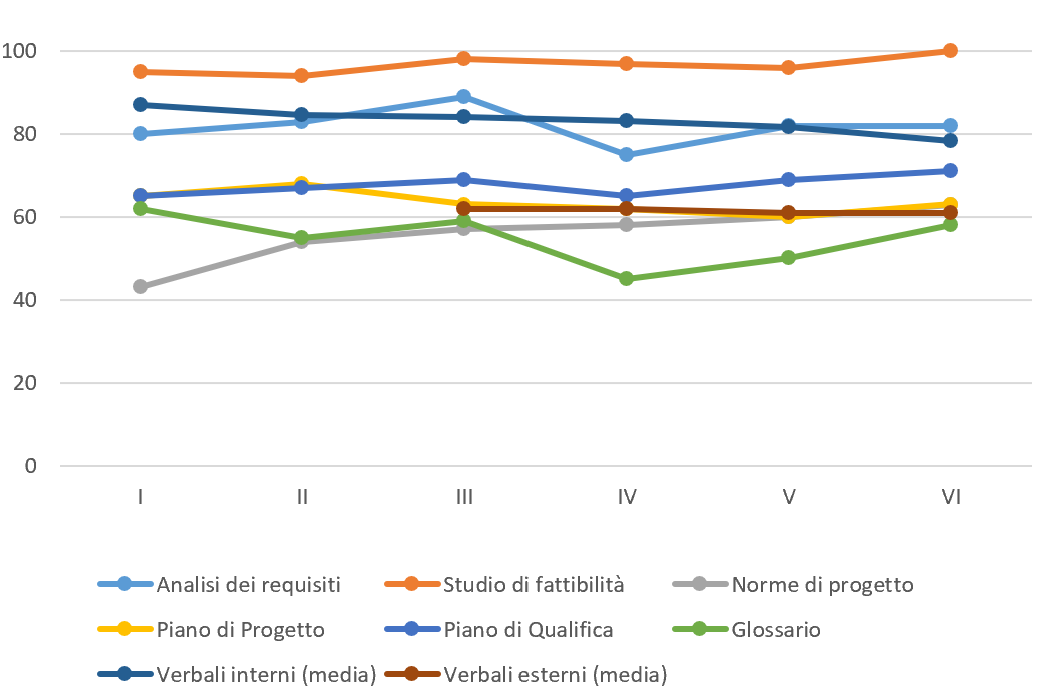
\includegraphics[width=\linewidth]{./img/grafici/2.png}	
	\caption{Indice di Gulpease revisione dei requisiti}	
\end{figure}
\subsubsection{Esito della revisione esterna}
Il gruppo ritiene poco soddisfacenti i risultati della revisione esterna per quanto riguarda la valutazione (24/30). 
Le correzioni comunicate attraverso colloqui e commenti alla valutazione ci hanno permesso di riflettere sui cambiamenti necessari da mettere in atto sia sui nostri prodotti che sul nostro way of working\glo.
Abbiamo quindi deciso di dare più importanza ai ruoli di verificatori e progettisti ritenendoli fondamentali per non ripetere più gli errori della precedente revisione e per sopperire alle carenze finora segnalate.
\end{itemize}  
Questa maggiore importanza non si rifletterà con un aumento delle ore dei ruoli di verificatore e progettista ma con un maggiore impegno da parte dei componenti del gruppo che andranno a svolgere i suddetti ruoli perché migliori la qualità e non il numero di queste ore.
\subsection{Revisione di progettazione (RP)}
\subsubsection{Riassunto delle attività di verifica}
In questo periodo abbiamo attuato le verifiche sui documenti, come nel precedente periodo. A queste abbiamo aggiunto le prime verifiche sulla codifica e sulla pianificazione per verificare che lo svolgimento del progetto procedesse senza intoppi.  
\paragraph{Analisi statica dei documenti}
L'analisi statica\glosp dei documenti ha portato alla produzione di una lista degli errori comuni ridotti rispetto alla revisione precedente. Questa lista deve essere aggiornata con le prossime analisi e andrà a facilitare il compito dei verificatori.
\subsubsection{Esiti delle verifiche} 
\paragraph{M01 Scostamento dei requisiti individuati} \mbox{}
\begin{longtable}[H!] {						
		>{}p{50mm}  		
		>{}p{8mm}
		>{}p{8mm}		
		>{}p{8mm}		
		>{}p{8mm}		
		>{}p{8mm}		
		>{}p{8mm}
		>{}p{8mm}
		>{}p{8mm}
		>{}p{8mm}
	}
\rowcolor{gray!50}
\textbf{} & \textbf{I} & \textbf{II} & \textbf{III} & \textbf{IV} & \textbf{V} & \textbf{VI} \TBstrut \\ [2mm]
\textbf{Scostamenti} & 3 & 3 & 3 & 3 & 3 & - \TBstrut \\ [2mm]
	\rowcolor{white}
\caption{M01 revisione di progettazione}
\end{longtable}
%\begin{figure}[H] 	
%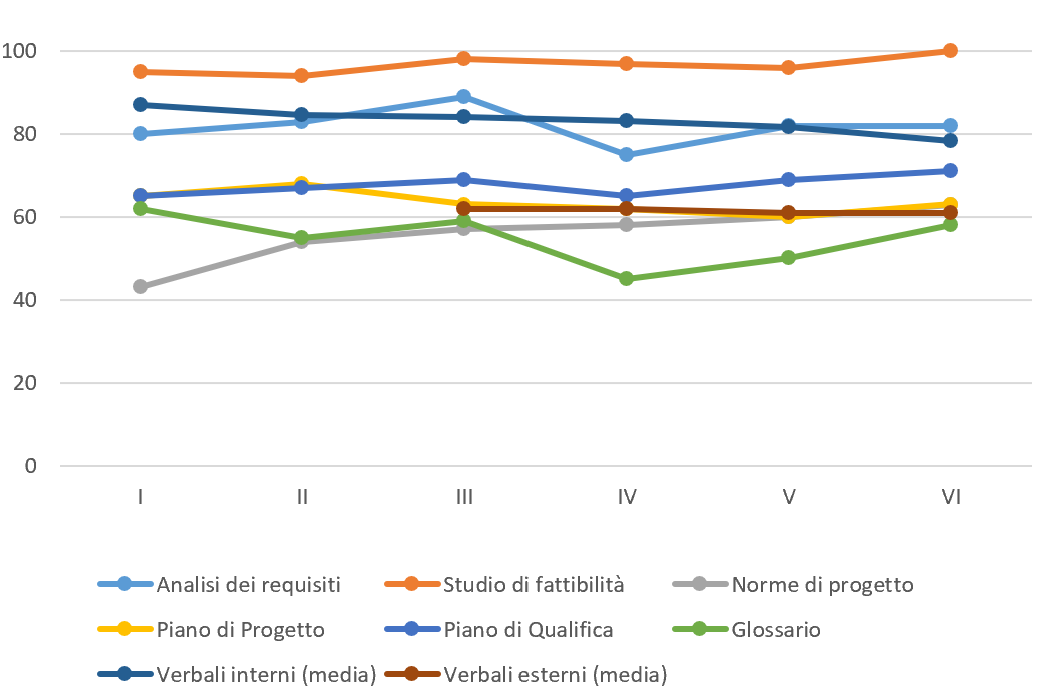
\includegraphics[width=\linewidth]{./img/grafici/2.png}	
%\caption{M01 revisione di progettazione}	
%\end{figure}
\paragraph{M06 Numero di parametri per metodo} \mbox{}
\begin{longtable}[H!] {						
		>{}p{50mm}  		
		>{}p{8mm}
		>{}p{8mm}		
		>{}p{8mm}		
		>{}p{8mm}		
		>{}p{8mm}		
		>{}p{8mm}
		>{}p{8mm}
		>{}p{8mm}
		>{}p{8mm}
	}
	\rowcolor{gray!50}
	\textbf{} & \textbf{I} & \textbf{II} & \textbf{III} & \textbf{IV} & \textbf{V} & \textbf{VI} \TBstrut \\ [2mm]
	\textbf{Numero di parametri} & - & - & 3 & 3 & 3 & - \TBstrut \\ [2mm]
	\rowcolor{white}
	\caption{M06 revisione di progettazione}
\end{longtable}
%\begin{figure}[H] 	
%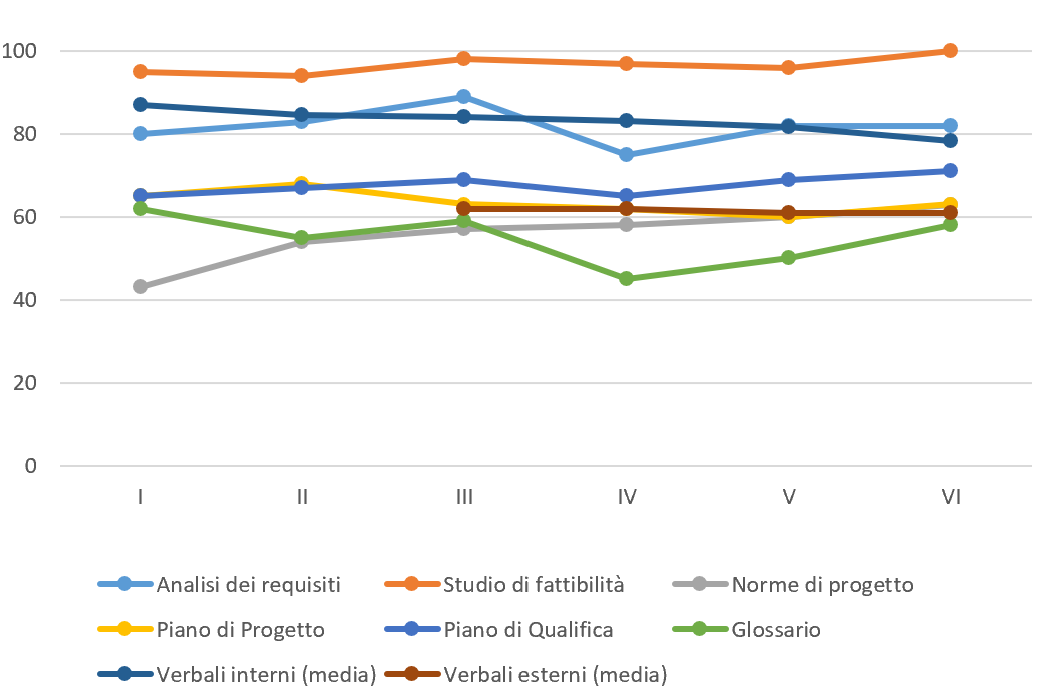
\includegraphics[width=\linewidth]{./img/grafici/2.png}	
%\caption{M06 revisione di progettazione}	
%\end{figure}
\paragraph{M07 Numero di metodi per classe} \mbox{}
\begin{longtable}[H!] {						
		>{}p{50mm}  		
		>{}p{8mm}
		>{}p{8mm}		
		>{}p{8mm}		
		>{}p{8mm}		
		>{}p{8mm}		
		>{}p{8mm}
		>{}p{8mm}
		>{}p{8mm}
		>{}p{8mm}
	}
	\rowcolor{gray!50}
	\textbf{} & \textbf{I} & \textbf{II} & \textbf{III} & \textbf{IV} & \textbf{V} & \textbf{VI} \TBstrut \\ [2mm]
	\textbf{Numero di metodi} & - & - & 3 & 3 & 3 & - \TBstrut \\ [2mm]
	\rowcolor{white}
	\caption{M07 revisione di progettazione}
\end{longtable}
%\begin{figure}[H] 	
%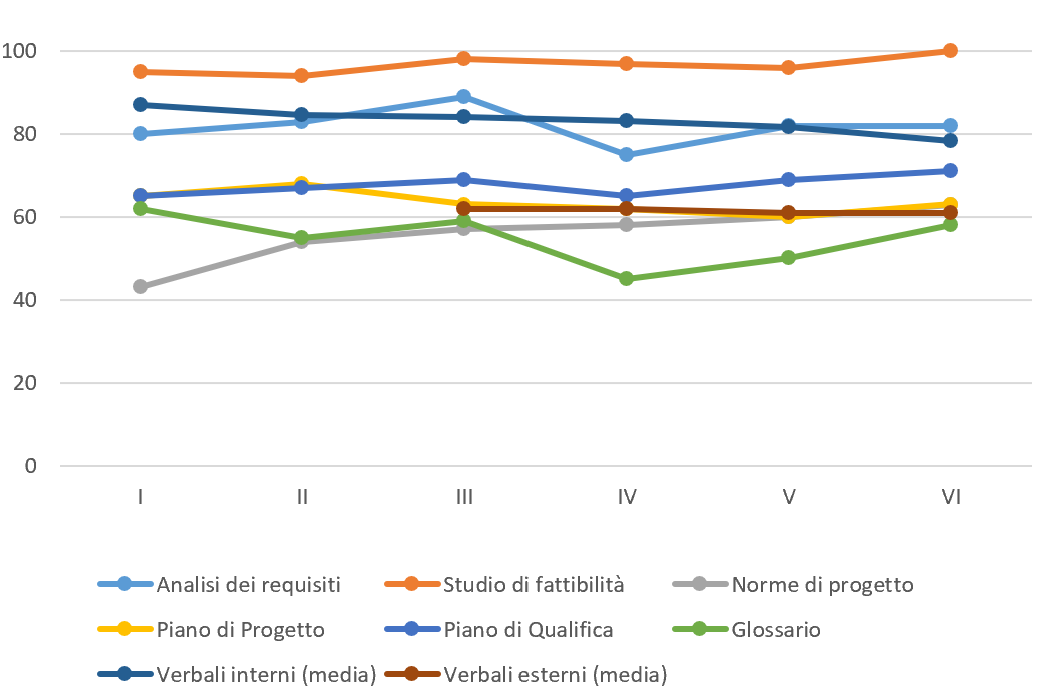
\includegraphics[width=\linewidth]{./img/grafici/2.png}	
%\caption{M07 revisione di progettazione}	
%\end{figure}
\paragraph{M08 Presenza di code smells} \mbox{}
\begin{longtable}[H!] {						
		>{}p{50mm}  		
		>{}p{8mm}
		>{}p{8mm}		
		>{}p{8mm}		
		>{}p{8mm}		
		>{}p{8mm}		
		>{}p{8mm}
		>{}p{8mm}
		>{}p{8mm}
		>{}p{8mm}
	}
	\rowcolor{gray!50}
	\textbf{} & \textbf{I} & \textbf{II} & \textbf{III} & \textbf{IV} & \textbf{V} & \textbf{VI} \TBstrut \\ [2mm]
	\textbf{Numero di code smells} & - & - & 3 & 3 & 3 & - \TBstrut \\ [2mm]
	\rowcolor{white}
	\caption{M08 revisione di progettazione}
\end{longtable}
%\begin{figure}[H] 	
%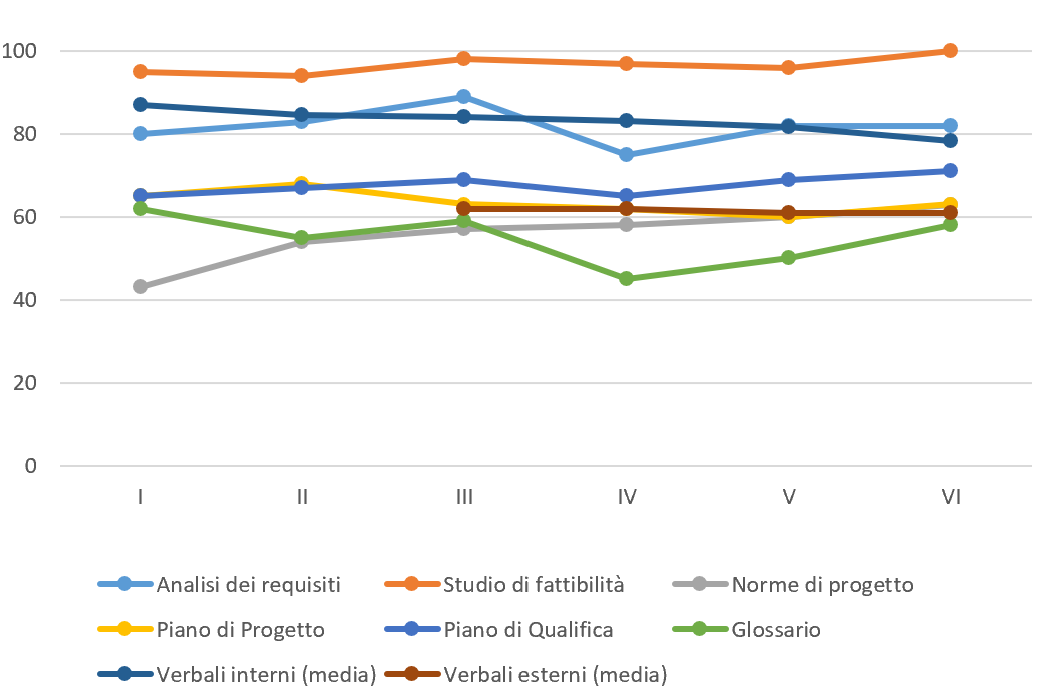
\includegraphics[width=\linewidth]{./img/grafici/2.png}	
%\caption{M08 revisione di progettazione}	
%\end{figure}
\paragraph{M09 Indice di Gulpease} \mbox{}
\begin{longtable} {						
		>{}p{50mm}  		
		>{}p{8mm}		
		>{}p{8mm}		
		>{}p{8mm}		
		>{}p{8mm}		
		>{}p{8mm}		
		>{}p{8mm}
		>{}p{8mm}
		>{}p{8mm}
		>{}p{8mm}				
	}			
	\rowcolor{gray!50}
	\textbf{Documento} & \textbf{I} & \textbf{II} & \textbf{III} & \textbf{IV} & \textbf{V} & \textbf{VI} \TBstrut \\ [2mm]
	\textbf{Analisi dei Requisiti} & 3 & 83 & 89 & 75 & 82 & - \TBstrut \\ [2mm]
	\textbf{Norme di Progetto} & 43 & 54 & 57 & 58 & 60 & - \TBstrut \\ [2mm]
	\textbf{Piano di Progetto} & 65 & 68 & 63 & 62 & 60 & - \TBstrut \\ [2mm]
	\textbf{Piano di Qualifica} & 65 & 67 & 69 & 65 & 69 & - \TBstrut \\ [2mm]
	\textbf{Glossario} & 62 & 55 & 59 & 45 & 50 & - \TBstrut \\ [2mm]
	\textbf{Verbali interni (media)} & 87 & 85 & 84 & 83 & 82 & - \TBstrut \\ [2mm]
	\textbf{Verbali esterni (media)} & - & - & 62 & 62 & 61 & - \TBstrut \\ [2mm]
	\rowcolor{white}
	\caption{M09 revisione di progettazione}
\end{longtable}
%\begin{figure}[H] 	
%	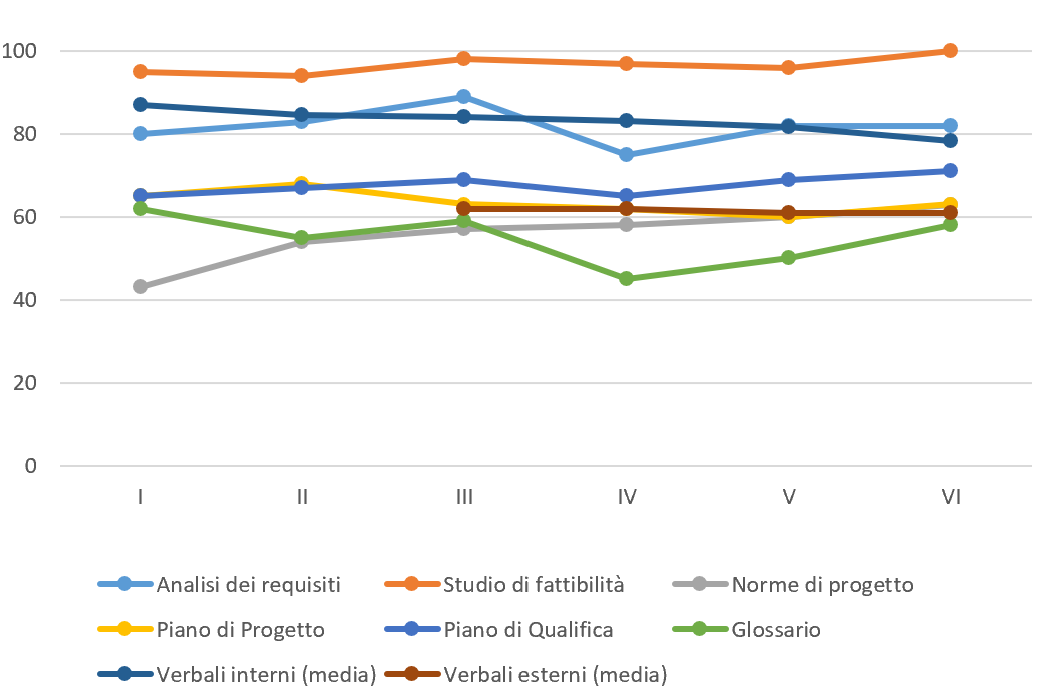
\includegraphics[width=\linewidth]{./img/grafici/2.png}	
%	\caption{M09 revisione di progettazione}	
%\end{figure}
\paragraph{M11 Budget at completion} \mbox{}
\begin{longtable}[H!] {						
		>{}p{50mm}  		
		>{}p{8mm}
		>{}p{8mm}		
		>{}p{8mm}		
		>{}p{8mm}		
		>{}p{8mm}		
		>{}p{8mm}
		>{}p{8mm}
		>{}p{8mm}
		>{}p{8mm}
	}
	\rowcolor{gray!50}
	\textbf{} & \textbf{I} & \textbf{II} & \textbf{III} & \textbf{IV} & \textbf{V} & \textbf{VI} \TBstrut \\ [2mm]
	\textbf{BAC} & 3 & 3 & 3 & 3 & 3 & - \TBstrut \\ [2mm]
	\rowcolor{white}
	\caption{M11 revisione di progettazione}
\end{longtable}
%\begin{figure}[H] 	
%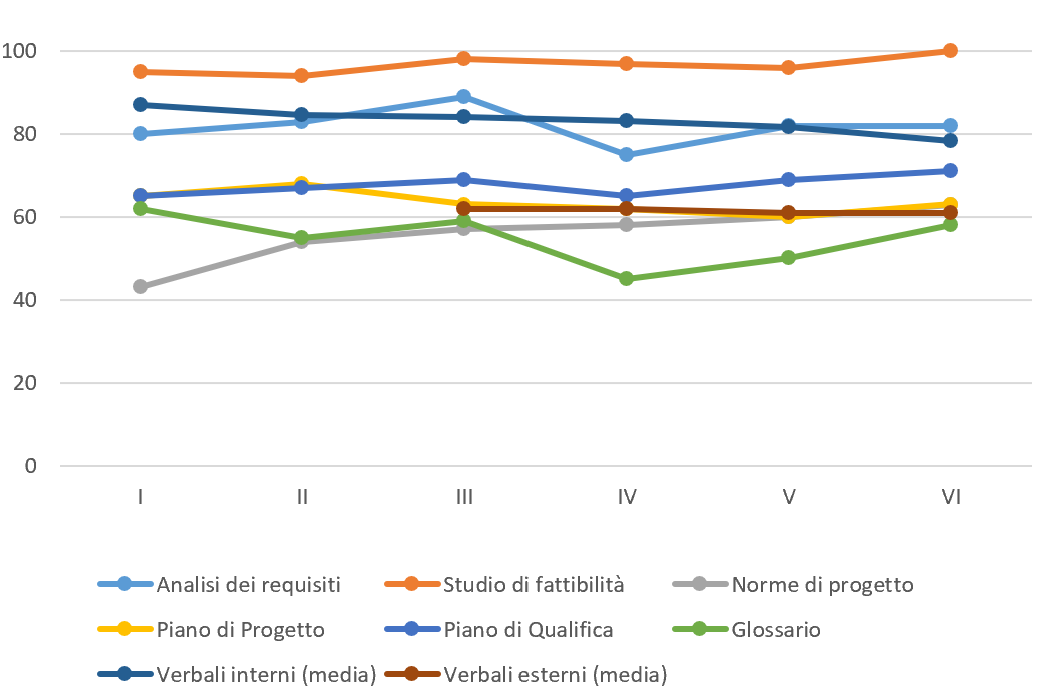
\includegraphics[width=\linewidth]{./img/grafici/2.png}	
%\caption{M11 revisione di progettazione}	
%\end{figure}
\paragraph{M12 Planned value} \mbox{}
\begin{longtable}[H!] {						
		>{}p{50mm}  		
		>{}p{8mm}
		>{}p{8mm}		
		>{}p{8mm}		
		>{}p{8mm}		
		>{}p{8mm}		
		>{}p{8mm}
		>{}p{8mm}
		>{}p{8mm}
		>{}p{8mm}
	}
	\rowcolor{gray!50}
	\textbf{} & \textbf{I} & \textbf{II} & \textbf{III} & \textbf{IV} & \textbf{V} & \textbf{VI} \TBstrut \\ [2mm]
	\textbf{PV} & 3 & 3 & 3 & 3 & 3 & - \TBstrut \\ [2mm]
	\rowcolor{white}
	\caption{M12 revisione di progettazione}
\end{longtable}
%\begin{figure}[H] 	
%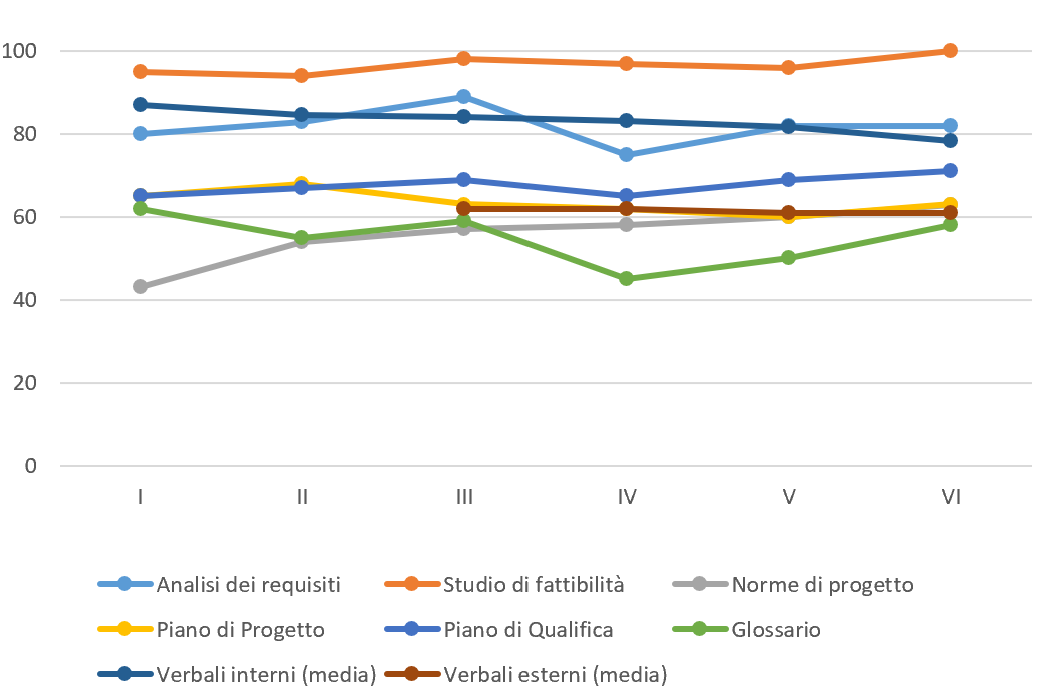
\includegraphics[width=\linewidth]{./img/grafici/2.png}	
%\caption{M12 revisione di progettazione}	
%\end{figure}
\paragraph{M13 Earned value} \mbox{}
\begin{longtable}[H!] {						
		>{}p{50mm}  		
		>{}p{8mm}
		>{}p{8mm}		
		>{}p{8mm}		
		>{}p{8mm}		
		>{}p{8mm}		
		>{}p{8mm}
		>{}p{8mm}
		>{}p{8mm}
		>{}p{8mm}
	}
	\rowcolor{gray!50}
	\textbf{} & \textbf{I} & \textbf{II} & \textbf{III} & \textbf{IV} & \textbf{V} & \textbf{VI} \TBstrut \\ [2mm]
	\textbf{EV} & 3 & 3 & 3 & 3 & 3 & - \TBstrut \\ [2mm]
	\rowcolor{white}
	\caption{M13 revisione di progettazione}
\end{longtable}
%\begin{figure}[H] 	
%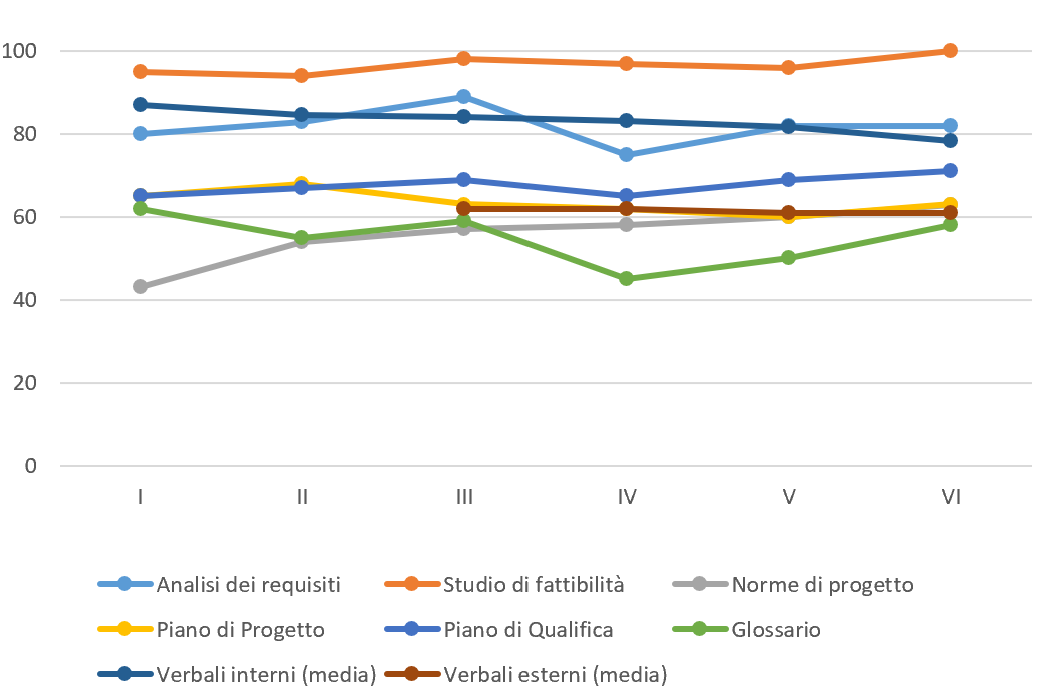
\includegraphics[width=\linewidth]{./img/grafici/2.png}	
%\caption{M13 revisione di progettazione}	
%\end{figure}
\paragraph{M14 Actual cost} \mbox{}
\begin{longtable}[H!] {						
		>{}p{50mm}  		
		>{}p{8mm}
		>{}p{8mm}		
		>{}p{8mm}		
		>{}p{8mm}		
		>{}p{8mm}		
		>{}p{8mm}
		>{}p{8mm}
		>{}p{8mm}
		>{}p{8mm}
	}
	\rowcolor{gray!50}
	\textbf{} & \textbf{I} & \textbf{II} & \textbf{III} & \textbf{IV} & \textbf{V} & \textbf{VI} \TBstrut \\ [2mm]
	\textbf{AC} & 3 & 3 & 3 & 3 & 3 & - \TBstrut \\ [2mm]
	\rowcolor{white}
	\caption{M14 revisione di progettazione}
\end{longtable}
%\begin{figure}[H] 	
%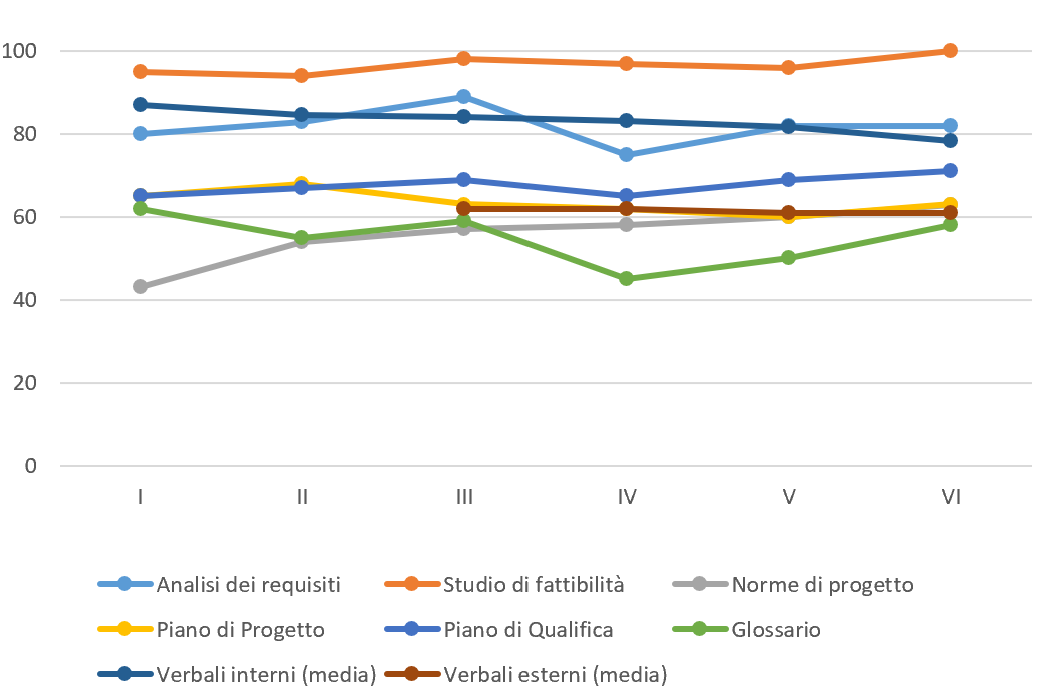
\includegraphics[width=\linewidth]{./img/grafici/2.png}	
%\caption{M14 revisione di progettazione}	
%\end{figure}
\paragraph{M15 Cost performance index} \mbox{}
\begin{longtable}[H!] {						
		>{}p{50mm}  		
		>{}p{8mm}
		>{}p{8mm}		
		>{}p{8mm}		
		>{}p{8mm}		
		>{}p{8mm}		
		>{}p{8mm}
		>{}p{8mm}
		>{}p{8mm}
		>{}p{8mm}
	}
	\rowcolor{gray!50}
	\textbf{} & \textbf{I} & \textbf{II} & \textbf{III} & \textbf{IV} & \textbf{V} & \textbf{VI} \TBstrut \\ [2mm]
	\textbf{CPI} & 3 & 3 & 3 & 3 & 3 & - \TBstrut \\ [2mm]
	\rowcolor{white}
	\caption{M15 revisione di progettazione}
\end{longtable}
%\begin{figure}[H] 	
%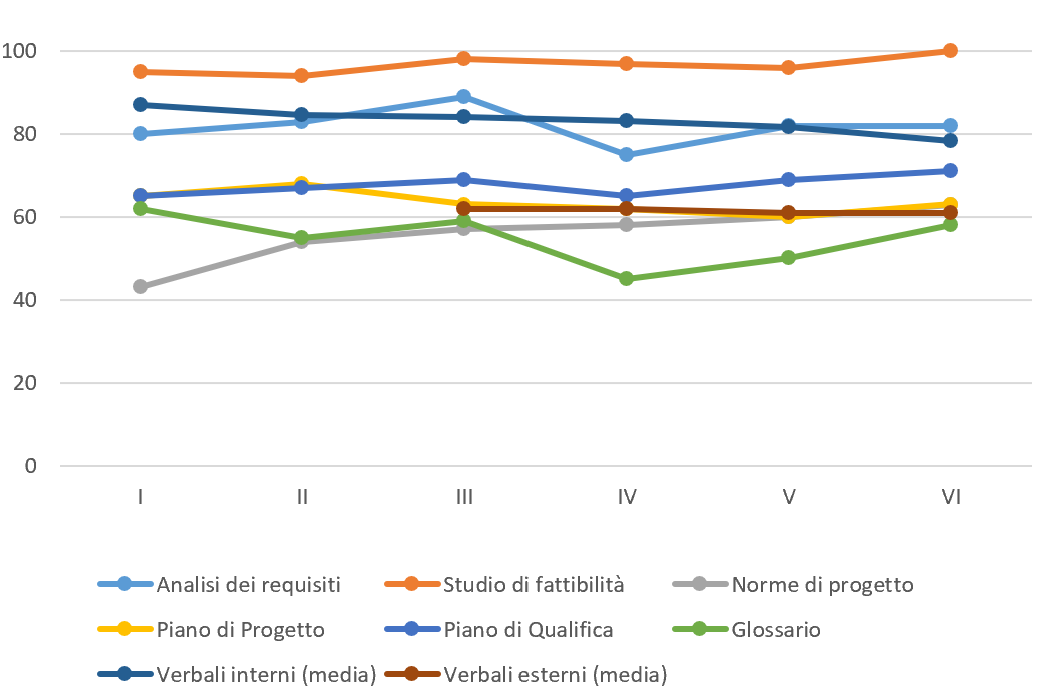
\includegraphics[width=\linewidth]{./img/grafici/2.png}	
%\caption{M15 revisione di progettazione}	
%\end{figure}
\paragraph{M16 Schedule performance index} \mbox{}
\begin{longtable}[H!] {						
		>{}p{50mm}  		
		>{}p{8mm}
		>{}p{8mm}		
		>{}p{8mm}		
		>{}p{8mm}		
		>{}p{8mm}		
		>{}p{8mm}
		>{}p{8mm}
		>{}p{8mm}
		>{}p{8mm}
	}
	\rowcolor{gray!50}
	\textbf{} & \textbf{I} & \textbf{II} & \textbf{III} & \textbf{IV} & \textbf{V} & \textbf{VI} \TBstrut \\ [2mm]
	\textbf{SPI} & 3 & 3 & 3 & 3 & 3 & - \TBstrut \\ [2mm]
	\rowcolor{white}
	\caption{M16 revisione di progettazione}
\end{longtable}
%\begin{figure}[H] 	
%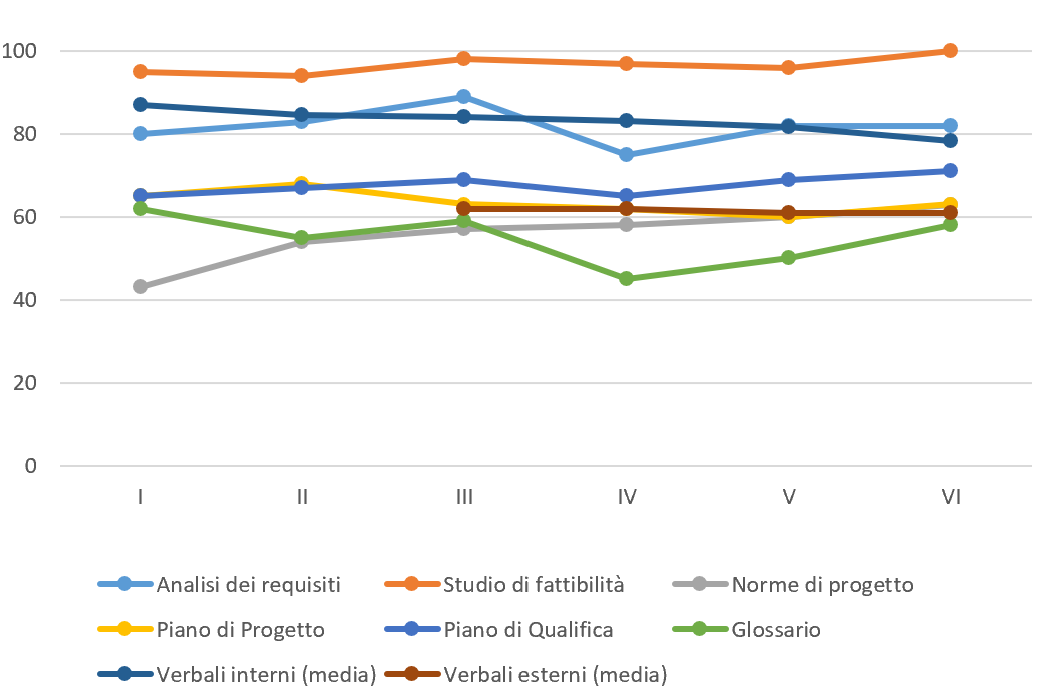
\includegraphics[width=\linewidth]{./img/grafici/2.png}	
%\caption{M16 revisione di progettazione}	
%\end{figure}
\paragraph{M17 Estimated cost at compltion} \mbox{}
\begin{longtable}[H!] {						
		>{}p{50mm}  		
		>{}p{8mm}
		>{}p{8mm}		
		>{}p{8mm}		
		>{}p{8mm}		
		>{}p{8mm}		
		>{}p{8mm}
		>{}p{8mm}
		>{}p{8mm}
		>{}p{8mm}
	}
	\rowcolor{gray!50}
	\textbf{} & \textbf{I} & \textbf{II} & \textbf{III} & \textbf{IV} & \textbf{V} & \textbf{VI} \TBstrut \\ [2mm]
	\textbf{EAC} & 3 & 3 & 3 & 3 & 3 & - \TBstrut \\ [2mm]
	\rowcolor{white}
	\caption{M17 revisione di progettazione}
\end{longtable}
%\begin{figure}[H] 	
%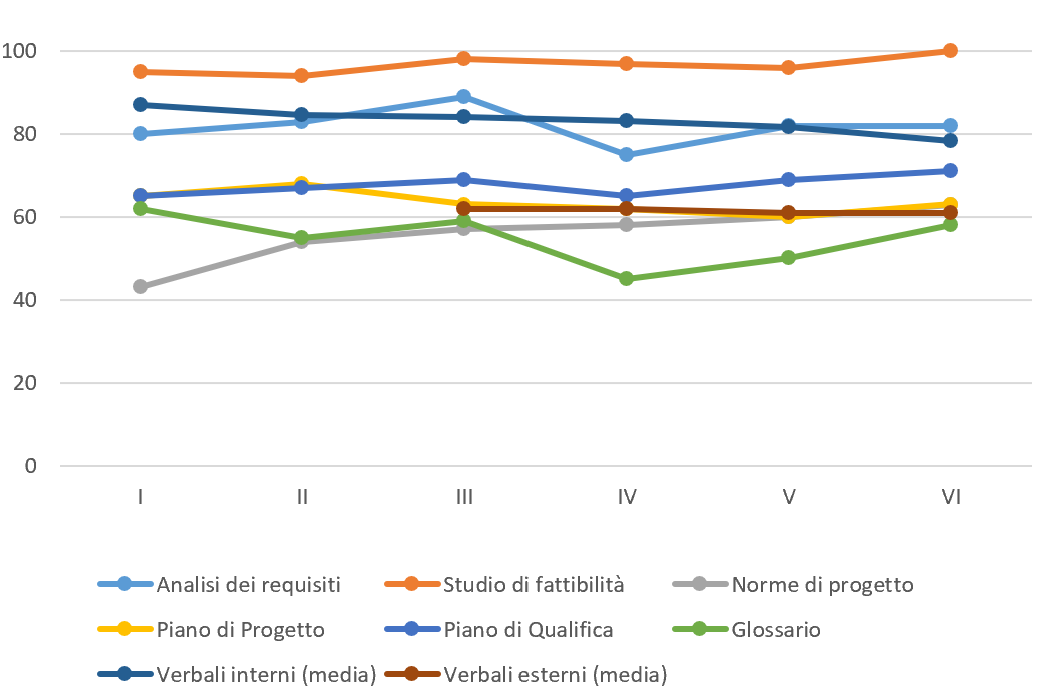
\includegraphics[width=\linewidth]{./img/grafici/2.png}	
%\caption{M17 revisione di progettazione}	
%\end{figure}
\paragraph{M18 Schedule at completion} \mbox{}
\begin{longtable}[H!] {						
		>{}p{50mm}  		
		>{}p{8mm}
		>{}p{8mm}		
		>{}p{8mm}		
		>{}p{8mm}		
		>{}p{8mm}		
		>{}p{8mm}
		>{}p{8mm}
		>{}p{8mm}
		>{}p{8mm}
	}
	\rowcolor{gray!50}
	\textbf{} & \textbf{I} & \textbf{II} & \textbf{III} & \textbf{IV} & \textbf{V} & \textbf{VI} \TBstrut \\ [2mm]
	\textbf{SAC} & 3 & 3 & 3 & 3 & 3 & - \TBstrut \\ [2mm]
	\rowcolor{white}
	\caption{M18 revisione di progettazione}
\end{longtable}
%\begin{figure}[H] 	
%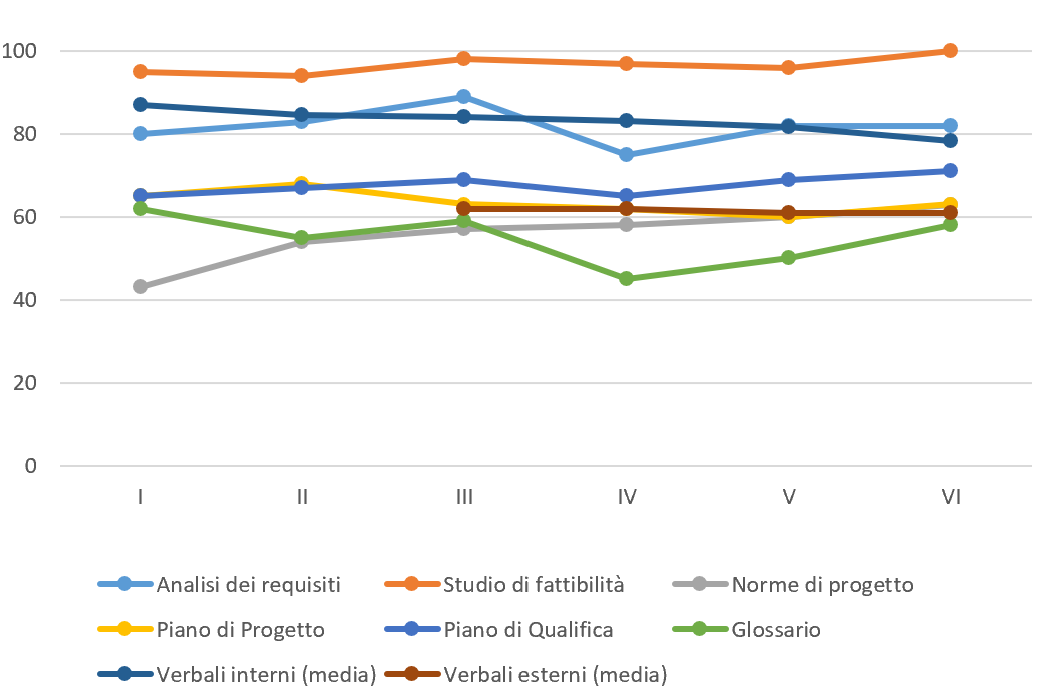
\includegraphics[width=\linewidth]{./img/grafici/2.png}	
%\caption{M18 revisione di progettazione}	
%\end{figure}
\paragraph{M19 Rischi non preventivati} \mbox{}
\begin{longtable}[H!] {						
		>{}p{50mm}  		
		>{}p{8mm}
		>{}p{8mm}		
		>{}p{8mm}		
		>{}p{8mm}		
		>{}p{8mm}		
		>{}p{8mm}
		>{}p{8mm}
		>{}p{8mm}
		>{}p{8mm}
	}
	\rowcolor{gray!50}
	\textbf{} & \textbf{I} & \textbf{II} & \textbf{III} & \textbf{IV} & \textbf{V} & \textbf{VI} \TBstrut \\ [2mm]
	\textbf{Rischi} & 3 & 3 & 3 & 3 & 3 & - \TBstrut \\ [2mm]
	\rowcolor{white}
	\caption{M19 revisione di progettazione}
\end{longtable}
%\begin{figure}[H] 	
%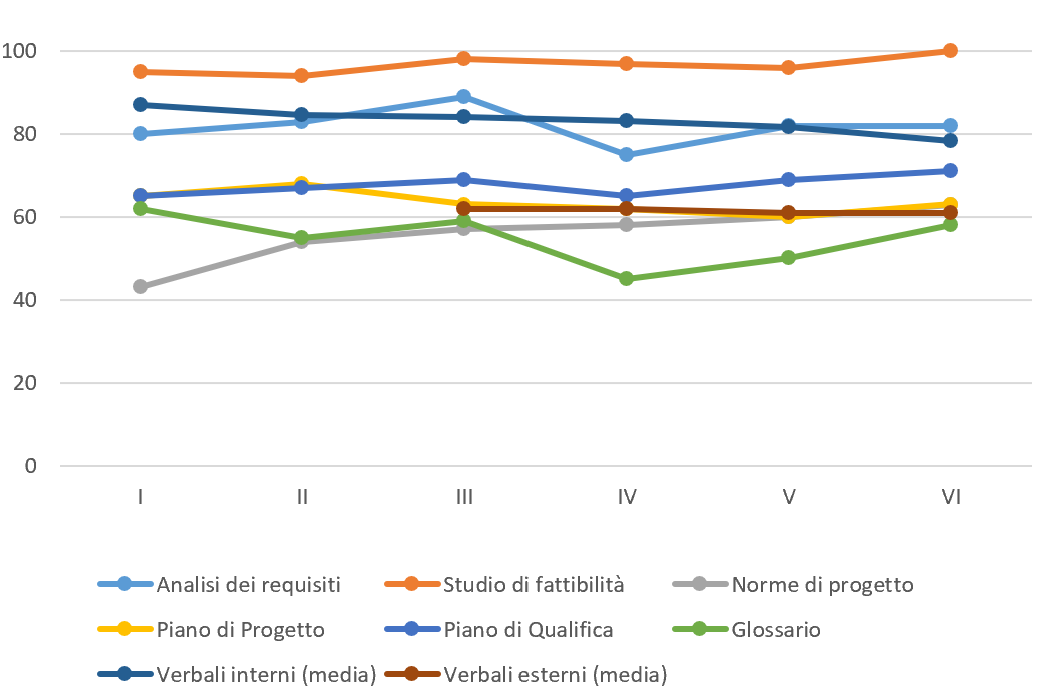
\includegraphics[width=\linewidth]{./img/grafici/2.png}	
%\caption{M19 revisione di progettazione}	
%\end{figure}
\paragraph{M20 Tempo medio risoluzione errori} \mbox{}
\begin{longtable}[H!] {						
		>{}p{50mm}  		
		>{}p{8mm}
		>{}p{8mm}		
		>{}p{8mm}		
		>{}p{8mm}		
		>{}p{8mm}		
		>{}p{8mm}
		>{}p{8mm}
		>{}p{8mm}
		>{}p{8mm}
	}
	\rowcolor{gray!50}
	\textbf{} & \textbf{I} & \textbf{II} & \textbf{III} & \textbf{IV} & \textbf{V} & \textbf{VI} \TBstrut \\ [2mm]
	\textbf{BAC} & 3 & 3 & 3 & 3 & 3 & - \TBstrut \\ [2mm]
	\rowcolor{white}
	\caption{M20 revisione di progettazione}
\end{longtable}
%\begin{figure}[H] 	
%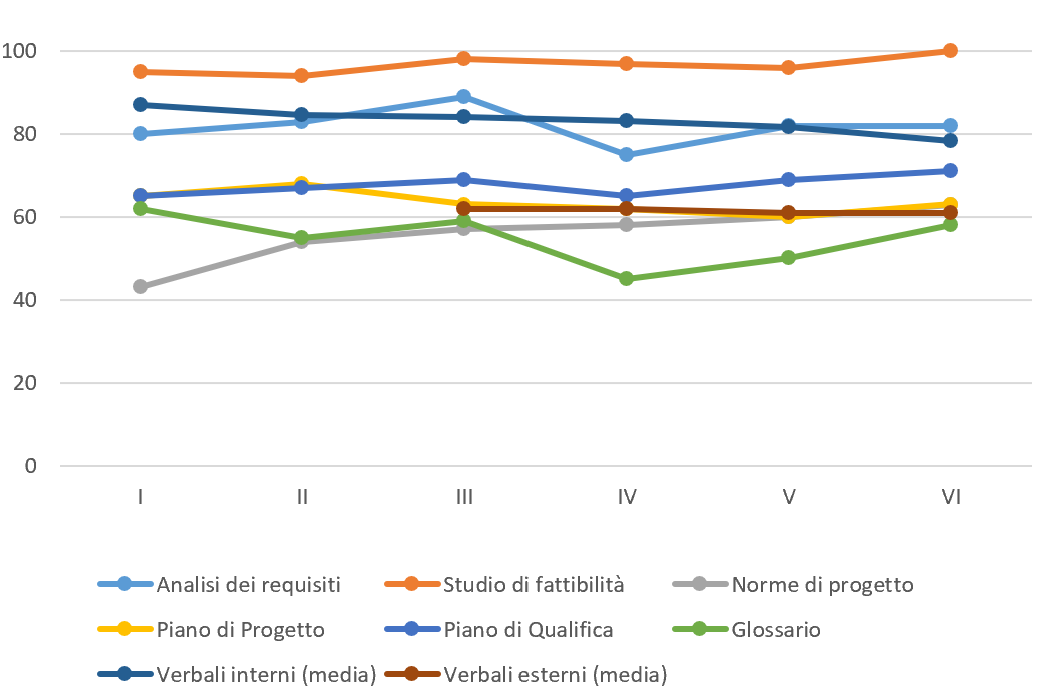
\includegraphics[width=\linewidth]{./img/grafici/2.png}	
%\caption{M20 revisione di progettazione}	
%\end{figure}
\paragraph{M21 Percentuale di requisiti obbligatori soddisfatti} \mbox{}
\begin{longtable}[H!] {						
		>{}p{50mm}  		
		>{}p{8mm}
		>{}p{8mm}		
		>{}p{8mm}		
		>{}p{8mm}		
		>{}p{8mm}		
		>{}p{8mm}
		>{}p{8mm}
		>{}p{8mm}
		>{}p{8mm}
	}
	\rowcolor{gray!50}
	\textbf{} & \textbf{I} & \textbf{II} & \textbf{III} & \textbf{IV} & \textbf{V} & \textbf{VI} \TBstrut \\ [2mm]
	\textbf{BAC} & 3 & 3 & 3 & 3 & 3 & - \TBstrut \\ [2mm]
	\rowcolor{white}
	\caption{M21 revisione di progettazione}
\end{longtable}
%\begin{figure}[H] 	
%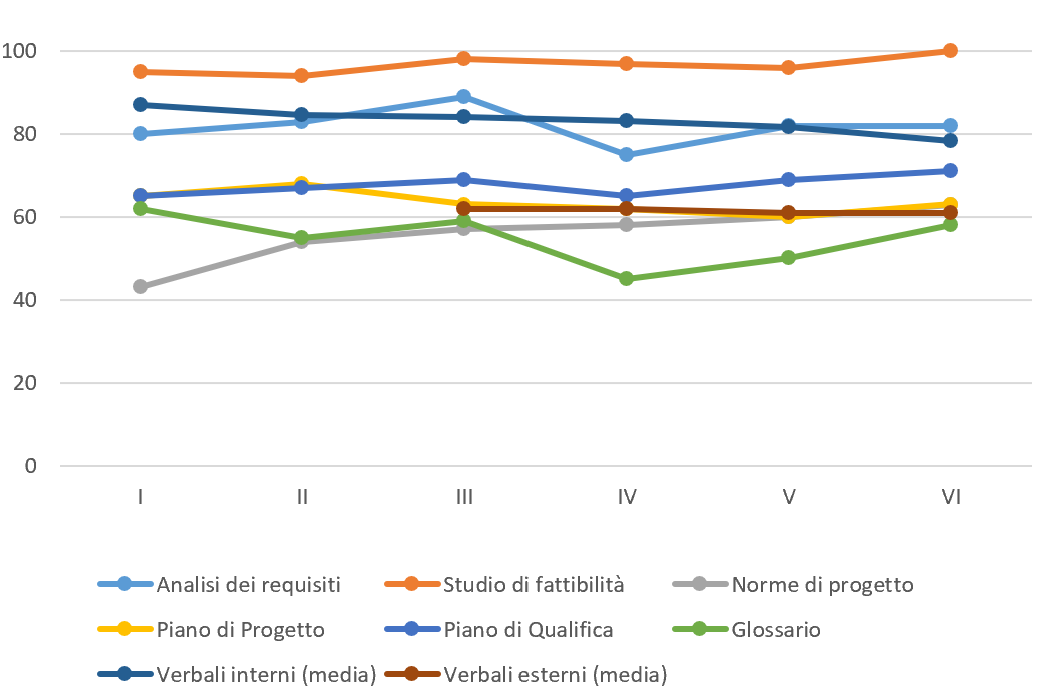
\includegraphics[width=\linewidth]{./img/grafici/2.png}	
%\caption{M21 revisione di progettazione}	
%\end{figure}
\paragraph{M22 Percentuale di requisiti desiderabili soddisfatti} \mbox{}
\begin{longtable}[H!] {						
		>{}p{50mm}  		
		>{}p{8mm}
		>{}p{8mm}		
		>{}p{8mm}		
		>{}p{8mm}		
		>{}p{8mm}		
		>{}p{8mm}
		>{}p{8mm}
		>{}p{8mm}
		>{}p{8mm}
	}
	\rowcolor{gray!50}
	\textbf{} & \textbf{I} & \textbf{II} & \textbf{III} & \textbf{IV} & \textbf{V} & \textbf{VI} \TBstrut \\ [2mm]
	\textbf{BAC} & 3 & 3 & 3 & 3 & 3 & - \TBstrut \\ [2mm]
	\rowcolor{white}
	\caption{M22 revisione di progettazione}
\end{longtable}
%\begin{figure}[H] 	
%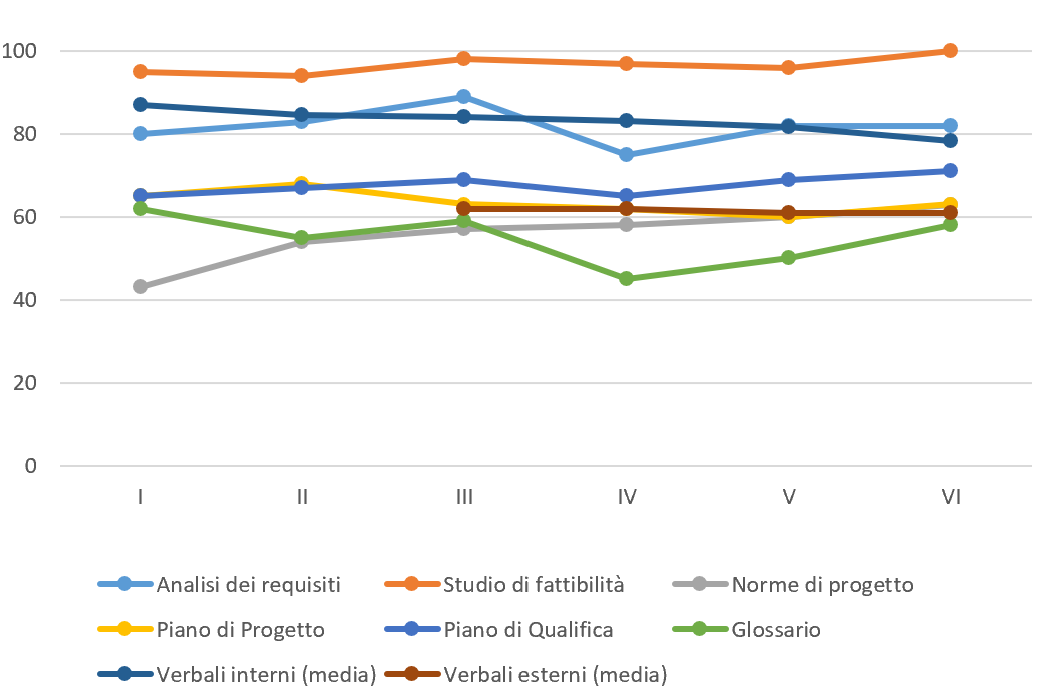
\includegraphics[width=\linewidth]{./img/grafici/2.png}	
%\caption{M22 revisione di progettazione}	
%\end{figure}
\paragraph{M23 Percentuale di requisiti opzionali soddisfatti} \mbox{}
\begin{longtable}[H!] {						
		>{}p{50mm}  		
		>{}p{8mm}
		>{}p{8mm}		
		>{}p{8mm}		
		>{}p{8mm}		
		>{}p{8mm}		
		>{}p{8mm}
		>{}p{8mm}
		>{}p{8mm}
		>{}p{8mm}
	}
	\rowcolor{gray!50}
	\textbf{} & \textbf{I} & \textbf{II} & \textbf{III} & \textbf{IV} & \textbf{V} & \textbf{VI} \TBstrut \\ [2mm]
	\textbf{BAC} & 3 & 3 & 3 & 3 & 3 & - \TBstrut \\ [2mm]
	\rowcolor{white}
	\caption{M23 revisione di progettazione}
\end{longtable}
%\begin{figure}[H] 	
%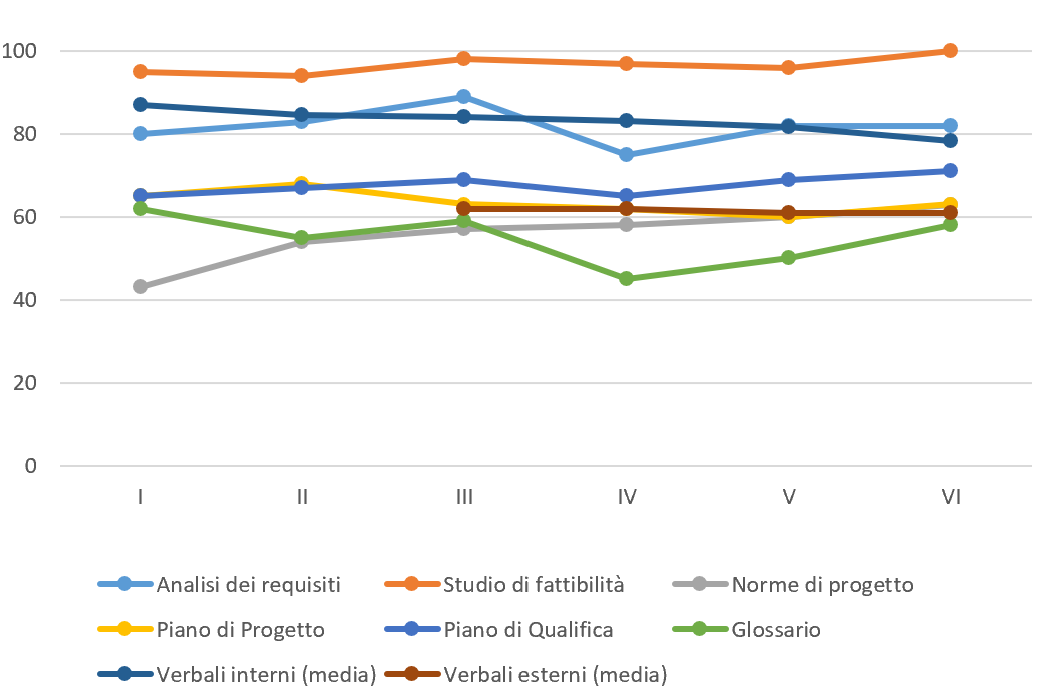
\includegraphics[width=\linewidth]{./img/grafici/2.png}	
%\caption{M23 revisione di progettazione}	
%\end{figure}
\paragraph{M30 Percentuale bug sistemati} \mbox{}
\begin{longtable}[H!] {						
		>{}p{50mm}  		
		>{}p{8mm}
		>{}p{8mm}		
		>{}p{8mm}		
		>{}p{8mm}		
		>{}p{8mm}		
		>{}p{8mm}
		>{}p{8mm}
		>{}p{8mm}
		>{}p{8mm}
	}
	\rowcolor{gray!50}
	\textbf{} & \textbf{I} & \textbf{II} & \textbf{III} & \textbf{IV} & \textbf{V} & \textbf{VI} \TBstrut \\ [2mm]
	\textbf{BAC} & 3 & 3 & 3 & 3 & 3 & - \TBstrut \\ [2mm]
	\rowcolor{white}
	\caption{M30 revisione di progettazione}
\end{longtable}
%\begin{figure}[H] 	
%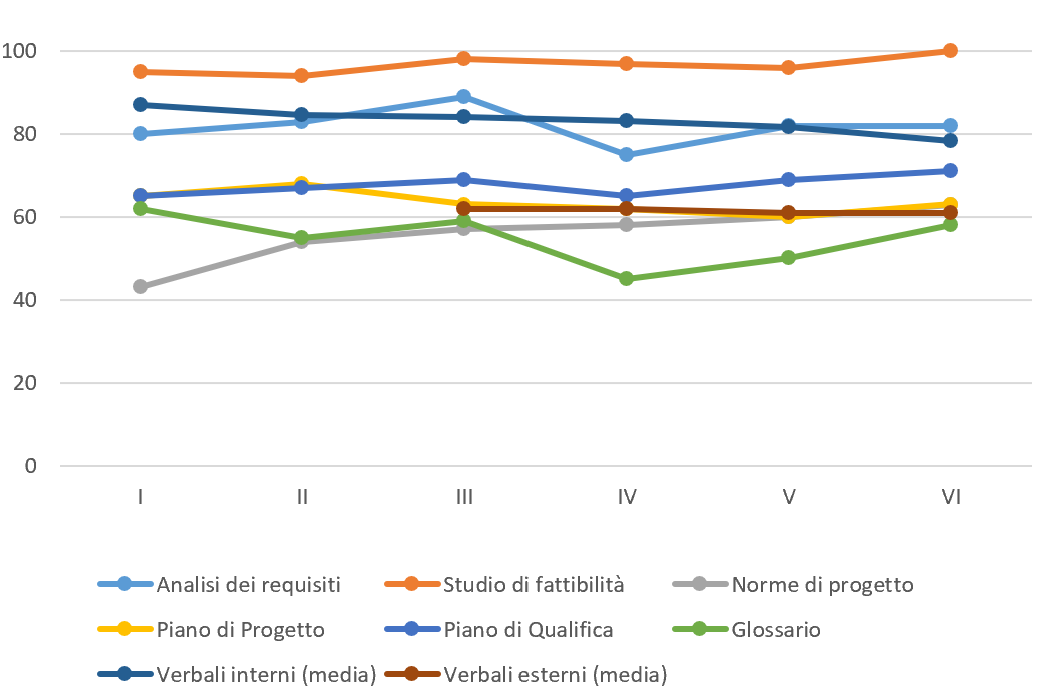
\includegraphics[width=\linewidth]{./img/grafici/2.png}	
%\caption{M30 revisione di progettazione}	
%\end{figure}
\paragraph{M10 Percentuale di metriche soddisfatte} \mbox{}
\begin{longtable}[H!] {						
		>{}p{50mm}  		
		>{}p{8mm}
		>{}p{8mm}		
		>{}p{8mm}		
		>{}p{8mm}		
		>{}p{8mm}		
		>{}p{8mm}
		>{}p{8mm}
		>{}p{8mm}
		>{}p{8mm}
	}
	\rowcolor{gray!50}
	\textbf{} & \textbf{I} & \textbf{II} & \textbf{III} & \textbf{IV} & \textbf{V} & \textbf{VI} \TBstrut \\ [2mm]
	\textbf{Numero di metodi} & - & - & 3 & 3 & 3 & - \TBstrut \\ [2mm]
	\rowcolor{white}
	\caption{M08 revisione di progettazione}
\end{longtable}
%\begin{figure}[H] 	
%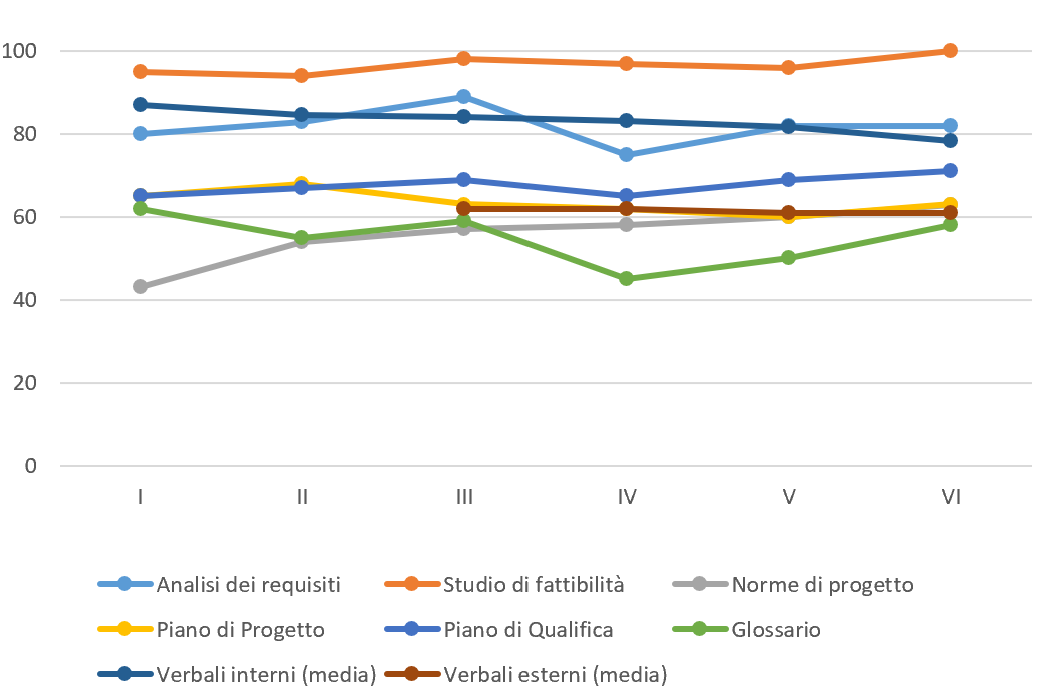
\includegraphics[width=\linewidth]{./img/grafici/2.png}	
%\caption{M08 revisione di progettazione}	
%\end{figure}


















\subsubsection{Revisioni generali}\mbox{}
\begin{longtable} {						
		>{}p{50mm}  		
		>{}p{8mm}		
		>{}p{8mm}		
		>{}p{8mm}		
		>{}p{8mm}		
		>{}p{8mm}		
		>{}p{8mm}
		>{}p{8mm}				
	}			
	\rowcolor{gray!50}
	\textbf{Metrica} & \textbf{RR} & \textbf{RP} & \textbf{RQ} & \textbf{RA} \TBstrut \\ [2mm]
	\textbf{Indice di Gulpease (media)} & 82 & - & - & - \TBstrut \\ [2mm]
	\textbf{M01} & 100 & - & - & - \TBstrut \\ [2mm]
	\textbf{Norme di Progetto} & 63 & - & - & - \TBstrut \\ [2mm]
	\textbf{Piano di Progetto} & 63 & - & - & - \TBstrut \\ [2mm]
	\textbf{Piano di Qualifica} & 71 & - & - & - \TBstrut \\ [2mm]
	\textbf{Glossario} & 58 & - & - & - \TBstrut \\ [2mm]
	\textbf{Verbali interni (media)} & 78 & - & - & - \TBstrut \\ [2mm]
	\textbf{Verbali esterni (media)}& 61 & - & - & - \TBstrut \\ [2mm]
	\rowcolor{white}
	\caption{Indice di Gulpease}
\end{longtable}
\begin{figure}[H] 	
	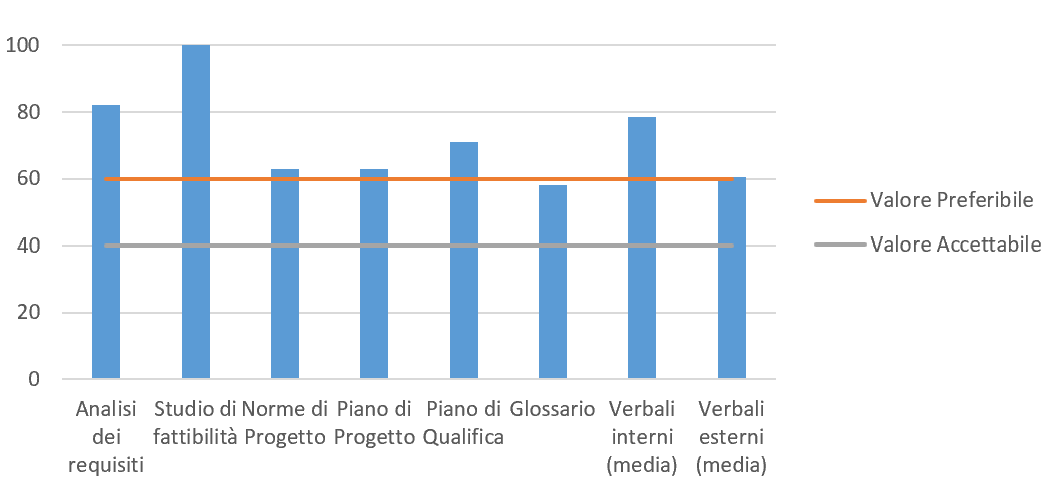
\includegraphics[width=\linewidth]{./img/grafici/1.png}	
	\caption{Indice di Gulpease}	
\end{figure}